The goal of query 2 is to identify outliers that consume significantly high amount of energy. The plug is counted as outlier if the median load of the plug is more than the median load of all the plugs in the system for a given sliding window (1 hr or 24 hrs).

\subsection{Architecture}
We are able to achieve a throughput of more than 670 thousand events per second using a single threaded C++ program in case of query 2.

\subsection{Median Algorithm}
In query 2, we have to calculate median of large amounts of data frequently. This leads to a clear trade off between computational complexity and accuracy of the median. We define a container which provides basic functionality of inserting a new element, deleting a given element and finally providing the approximate median for currently existing data in the container. We first insert all the elements into the container corresponding to the sliding window. Every time we slide by 1 sec, we perform at most 2 operations. We delete the oldest event if it exists and insert the latest event in the window. Every insert and/or delete operation is followed by computation of median. We, therefore, want to minimize the complexity of median calculation. We, now, propose an algorithm to compute median which takes constant time for every operation in the given scenario with very low relative error.

The basic idea is to construct a histogram of the data using fixed number of bins (M-1). The histogram is then queried to find median of the data. We sort the first M distinct values inserted into the container and use them in order to build up the (M-1) bins. Every $i^{th}$ inserted value corresponds to the starting of $i^{th}$ bin and every bin is associated with a frequency. Frequency denotes the frequency of the data greater and equal to $i^{th}$ lowest value (including) and less than $(i+1)^{th}$ lowest value (excluding) among M inserted value into the container. We also store the index of the bin containing the median after an insertion or deletion is performed, cumulative sum of the frequencies upto and including the bin in which median resides and the total number of values inserted into the container.

Every time a new value is inserted, the frequency of the corresponding bin is incremented. On the other hand, if a value is to be deleted, the frequency of the corresponding bin is decremented. At the time of insertion or deletion, we also modify the variable storing the index of the bin having the current median and accordingly the cumulative sum. The corresponding bin to insert/delete can be found in $\log(M)$ order complexity where (M-1) represents the number of bins. We handle below cases as follows-
\begin{itemize}
\item If frequency of a bin becomes significantly higher than some constant times the average bin frequency, we split the bin into two bins. Every new bin is given half of the frequency of the original bin. The range of values is also equally divided between 2 bins.
\item If frequency of a bin reaches to zero, we simply delete the bin.
\item If an inserted value is less than the lowest value or higher than the highest value present in the median container, we create another bin starting with the inserted value.
\item If number of bins are higher than the maximum allowed number of bins, we merge 2 bins. These 2 consecutive bins are chosen such that they have minimum total frequency than any other two consecutive bins. The frequency of the higher bin is added to the frequency of the lower bin and the higher bin is deleted.
\end{itemize}

We implemented median container using an array. Array provides the flexibility of binary search which is required to be done very frequently in our case. We keep two empty memory slots on both sides of the array, which simplifies an insertion of a new bin in case of inserted value not being in the existing range of values. When a new bin is inserted/merged in the middle of the array, we shift the rest of the array to fill up the void.  We used low level operation \textit{memmove} provided by cstring library in C++, in order to speed up the shift operation.

In this case we need to compute the median every time we receive an event. So every insert or deletion or both will be followed by a call to the \textit{getMedian} function of the container. We, therefore, used this nature of the problem, and optimized the asymptotic complexity of \textit{getMedian} to O(1). We modify the variable storing the index to the bin having the current median, at the time of insert and delete only.

\begin{table}[h]
\begin{center}
\begin{tabular}{|c|c|c|}
\hline 
 & \textbf{Worst Case} & \textbf{Average Case} \\ 
\hline 
\textbf{insert} & O(M) & O($\log(M)$) \\
\hline 
\textbf{delete} & O(M) & O($\log(M)$) \\
\hline 
\textbf{getMedian} & O(1) & O(1) \\ 
\hline 
\end{tabular} 
\end{center}
\end{table}

\subsection{Relative Error for Median Container}
In this case, we did 1000 experiments, each inserting 50000 values into the container. The CDF is plotted in the following figure.

\begin{figure}[h]
\begin{center}
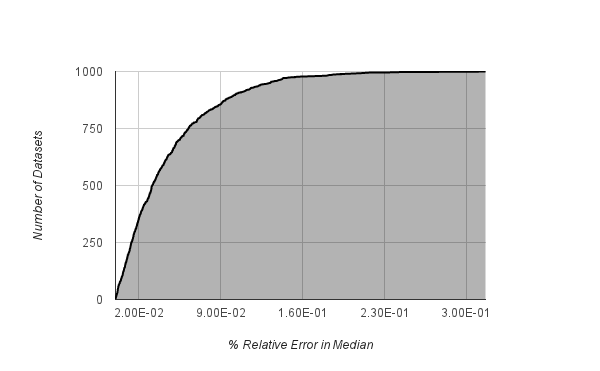
\includegraphics[scale=0.4]{img/relative_error}
\end{center}
\end{figure}

\subsection{Choosing Number of Bins}
We did experiments with the median container in order to figure out an optimum number of bins. Number of bins affect the accuracy of the computed median. We used 10 datasets generated randomly with different median and variance. We used different number of bins ranging from 100 to 2000 for each dataset and calculated relative error in each case.

\begin{figure}[h]
\begin{center}
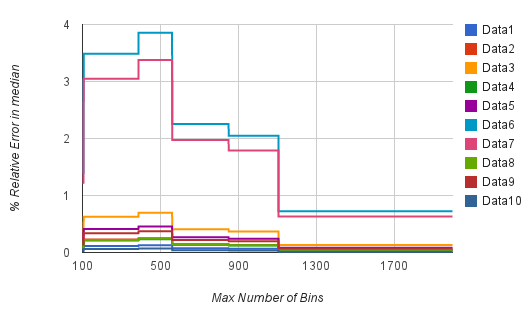
\includegraphics[scale=0.4]{img/bin_size_experiment}
\end{center}
\end{figure}

\subsection{S Container}
We have to compute the number of plugs in a house having higher median load than the global median load (median load of all the plugs in the system). In order to efficiently compute it, we defined another container called S container. S container stores median values of all the plugs in a house and evaluate the number of plugs higher than the global median. It provides basic operation of inserting (replacing) a newly computed plug median for the house, and finding out number of plugs which have higher median load than the global median (getNumOfLargeNum).

The issue here is, that we don't know number of plugs in a house before hand. It has to be acquired as the system makes progress. Hence, we had to use a map (key-value storage) in order to store the data but that leads to O(K) complexity of the \textit{getNumOfLargeNum} operation where K is the total number of plugs in a house. We avoided this by again using an array and stored all the data in sorted order with key being the plug median. When a new value is to be inserted, we require the old plug median in order to search the location of the plug data in the array. As soon as we find the location, we replace the new median with the old median and modify the location such that the array is sorted again.

The asymptotic complexity of this is also O(K) but in the given scenario, momentous change in median values are unlikely. It will take finite number of more than one steps which will lead to significant change in the median values. In such a case, very little movement will be required while sorting the array after an insertion is performed. On the other hand, \textit{getNumOfLargeNum} operation will always be $\log(K)$.

Also, we do not store the whole measurement (16 byte) in the array but just the pointers (4 byte) to those measurement, which leads to even less amount of shift in the data. We use \textit{memmove} operation provided by CString library of C++, rather than manual copying of the array to increase the performance of the container.

\subsection{Window Linked List}
We keep a linked list to store all the events occurred in a given window (1 hr and 24 hr). Every new event coming into the window is appended at the front and every event leaving the window is deleted from the end. In case of no missing event, every new event leads to an insertion of the latest arrived event at the front and deletion of the oldest event at the end of the linked list.


 In case of missing data, no events are appended or deleted from the window. The algorithm is triggered whenever a new event is received. The window is, then, shifted one event by one event until the latest received event enters the window and becomes the last event of the window. We don't slide any further.

As soon as we receive a new event, we start removing events from the end of the linked list one by one. Every time we delete an event, we compute the median of the plug corresponding to the deleted event. We also compute the global median (median of all the data of all the plugs in the system). Any change in global median requires computation for all houses i.e. we compute whether the number of plugs in a house having median greater than the global median has changed, for every house. Any change in the percentage leads to an output event. If global median is same, we simply look at the house of the plug corresponding to the deleted event only. We compute the number of plugs having median bigger than the global median for the house. Change in the percentage here, leads to another output event. The output event is associated to the window beginning at 1 higher timestamp than the deleted event (ts+1) to (ts+legnth(window)).


